\chapter{Résultats, benchmark et analyse}

\chapintro
Ce chapitre présente les résultats dans l'ordre de la démarche : la fiabilité de la population, la santé des roulements, puis la comparaison des sept méthodes de pronostic. Il se termine par la validation sur données simulées, l'explicabilité et le tableau de bord.

\section{Fiabilité de la population}

\subsection{Choix de la loi par la vraisemblance}
Le tableau~\ref{tab:lois} compare les quatre lois ajustées par maximum de vraisemblance, en tenant compte des 11 roulements censurés. Les trois lois à deux paramètres sont presque équivalentes (écart d'AIC inférieur à 2) ; la log-normale est à peine meilleure. Nous gardons la \textbf{loi de Weibull}, la référence en fiabilité, parce que son paramètre $\beta$ s'interprète directement (usure ou non) et donne le B10 par une formule simple.

\begin{table}[H]
\centering\small
\begin{tabular}{lccc}
\toprule
Loi & Paramètres & Log-vraisemblance & AIC \\
\midrule
Exponentielle & 1 & $-44{,}35$ & 90,70 \\
\textbf{Weibull} & 2 & $-42{,}98$ & 89,95 \\
Log-normale & 2 & $-42{,}65$ & 89,31 \\
Log-logistique & 2 & $-42{,}98$ & 89,96 \\
\bottomrule
\end{tabular}
\caption[Comparaison des lois par la vraisemblance]{Comparaison des lois de durée de vie (maximum de vraisemblance avec censure).}
\label{tab:lois}
\end{table}

La figure~\ref{fig:vraisemblance} montre les lois face à l'estimateur de Kaplan-Meier, et la surface de vraisemblance de Weibull : le maximum est atteint en $\beta = 1{,}85$ et $\eta = 422$ min, mais la région de confiance à 95 \% est très large. Le test du rapport de vraisemblance ($\beta = 1$ contre $\beta$ libre) donne $p = 0{,}097$ : avec seulement 6 défaillances, on ne peut pas \emph{prouver} l'usure au seuil de 5 \%. L'intervalle bootstrap de $\beta$, de 1,31 à 3,37, reste pourtant au-dessus de 1 : l'usure est probable.

\begin{figure}[H]
\centering
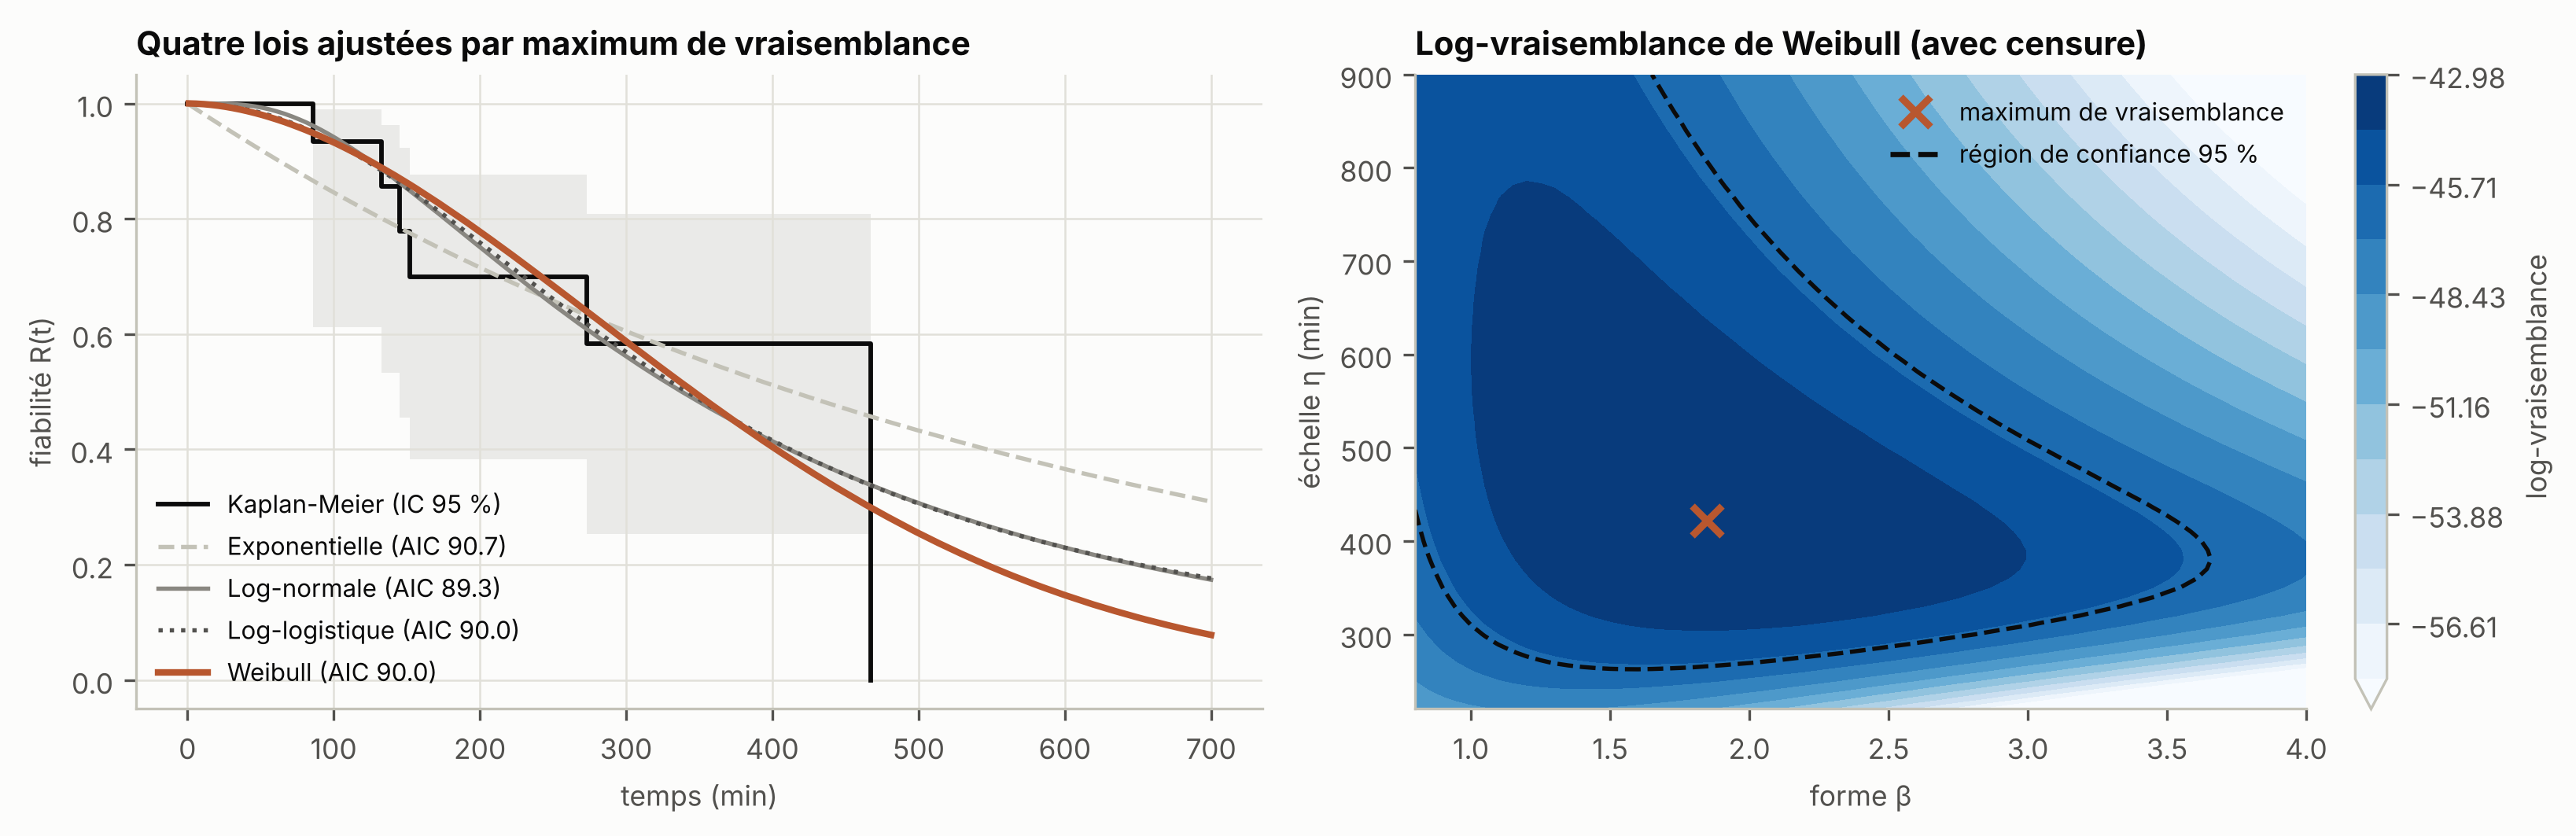
\includegraphics[width=\linewidth]{figures/fig18_vraisemblance.png}
\caption[Lois ajustées et surface de vraisemblance]{À gauche : quatre lois ajustées face à Kaplan-Meier. À droite : log-vraisemblance de Weibull, son maximum et la région de confiance à 95 \%.}
\label{fig:vraisemblance}
\end{figure}

\subsection{Indicateurs de fiabilité : B10, B50 et MTTF}
Le tableau~\ref{tab:fiabilite} donne les indicateurs, avec leurs intervalles de confiance à 95 \% obtenus par bootstrap. Un roulement sur dix casse avant 125 min et la moitié avant 346 min. Les intervalles sont larges : c'est le prix de 17 roulements seulement. La figure~\ref{fig:fiabilite} montre que le taux de défaillance augmente avec l'âge, et que le B10 conditionnel d'un roulement sain diminue quand il vieillit.

\begin{table}[H]
\centering\small
\begin{tabular}{lcc}
\toprule
Indicateur & Valeur & IC 95 \% (bootstrap) \\
\midrule
Forme $\beta$ & 1,85 & [1,31 ; 3,37] \\
Échelle $\eta$ & 422 min & [261 ; 732] min \\
MTTF & 375 min & [232 ; 666] min \\
B10 & 125 min & [78 ; 234] min \\
B50 (médiane) & 346 min & [219 ; 573] min \\
L10 des catalogues (conditions 1 / 2 / 3) & 556 / 524 / 341 min & — \\
\bottomrule
\end{tabular}
\caption[Indicateurs de fiabilité]{Indicateurs de fiabilité de la population (loi de Weibull).}
\label{tab:fiabilite}
\end{table}

\begin{figure}[H]
\centering
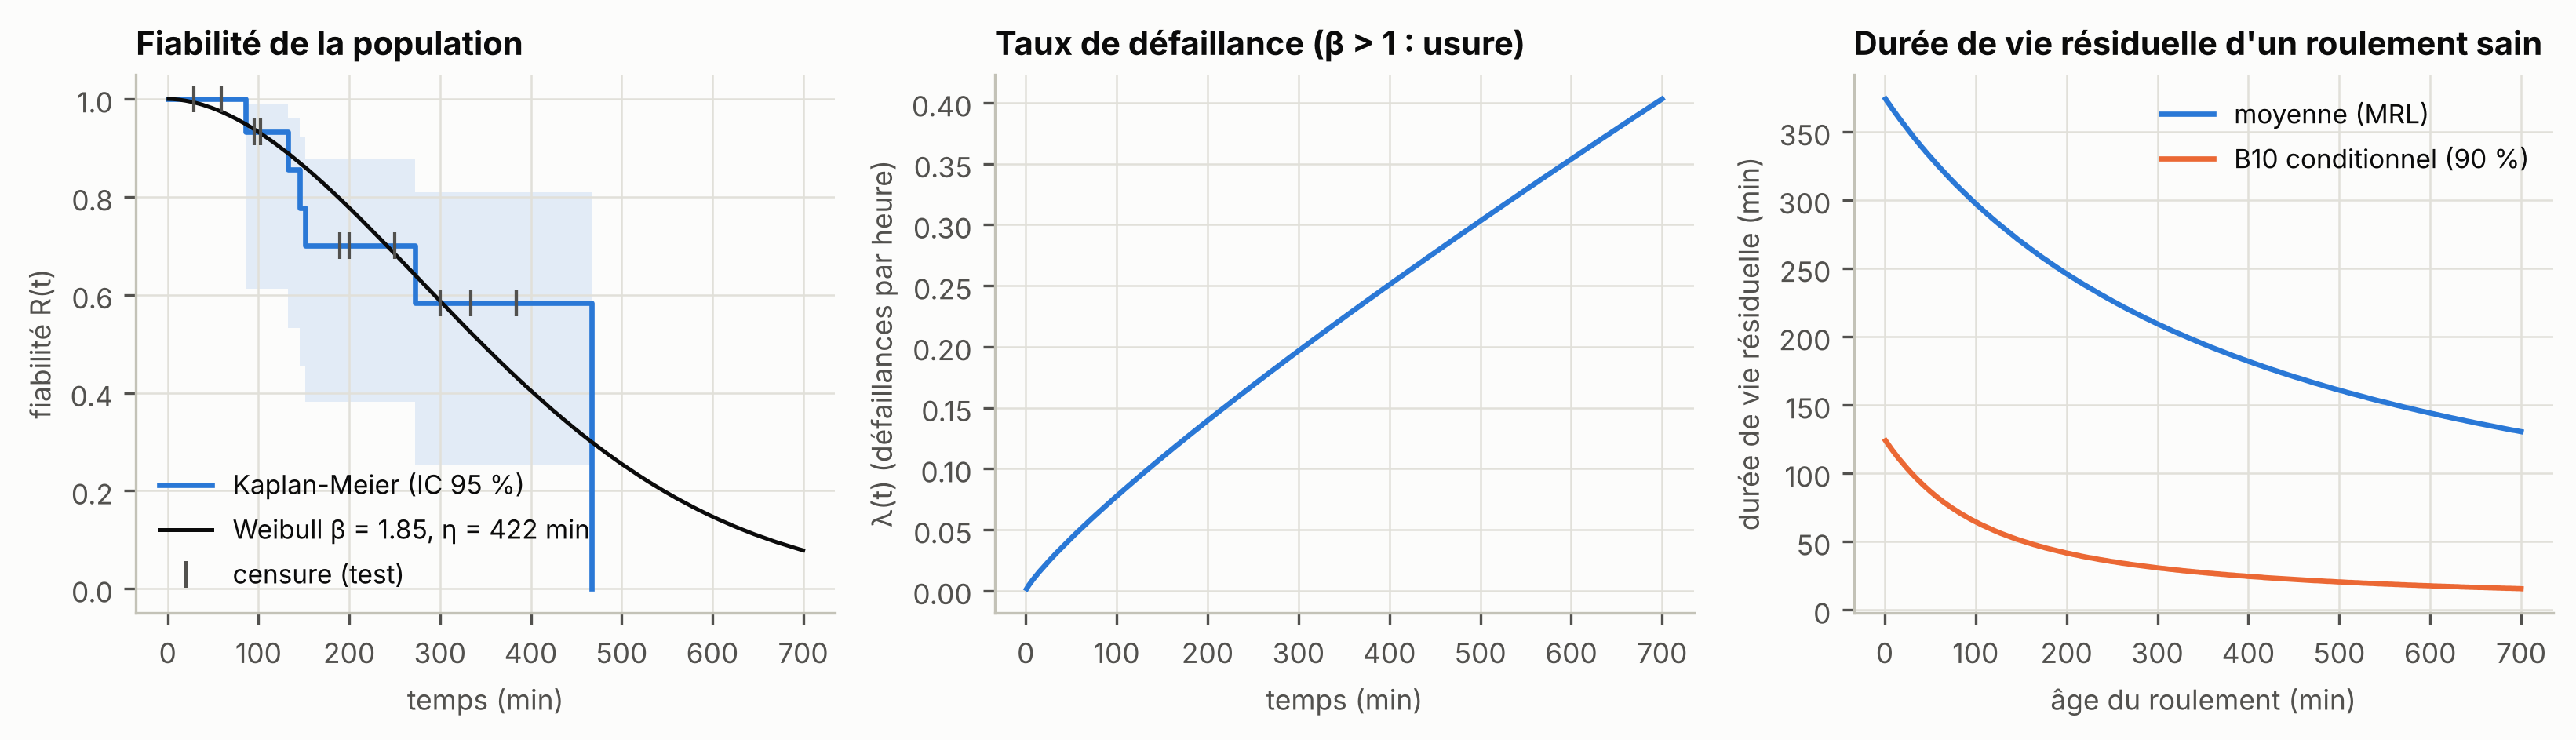
\includegraphics[width=\linewidth]{figures/fig04_fiabilite.png}
\caption[Fiabilité, taux de défaillance et B10 conditionnel]{Fiabilité de la population : Kaplan-Meier et Weibull, taux de défaillance, durée de vie résiduelle d'un roulement sain.}
\label{fig:fiabilite}
\end{figure}

La plupart des roulements cassent bien avant leur L10 (figure~\ref{fig:durees}) : la formule des catalogues ne s'applique pas à ces essais accélérés, ce que notent aussi les organisateurs du challenge \cite{phm2012challenge}.

\subsection{Ajout de covariables}
La figure~\ref{fig:covariables} ajoute la charge comme covariable (modèle AFT). \textbf{Un kilonewton de plus multiplie la durée de vie par 0,40} ($p = 0{,}042$), et l'AIC baisse de 90,0 à 88,3 : la covariable améliore le modèle. Le B10 passe de 175 min sous la condition 1 à 69 min sous la condition 3. La vitesse ($p = 0{,}033$) et la durée L10 ($p = 0{,}049$) donnent des conclusions semblables. Attention : la vitesse baisse quand la charge monte, et il n'y a que trois conditions ; les deux effets sont donc mélangés.

\begin{figure}[H]
\centering
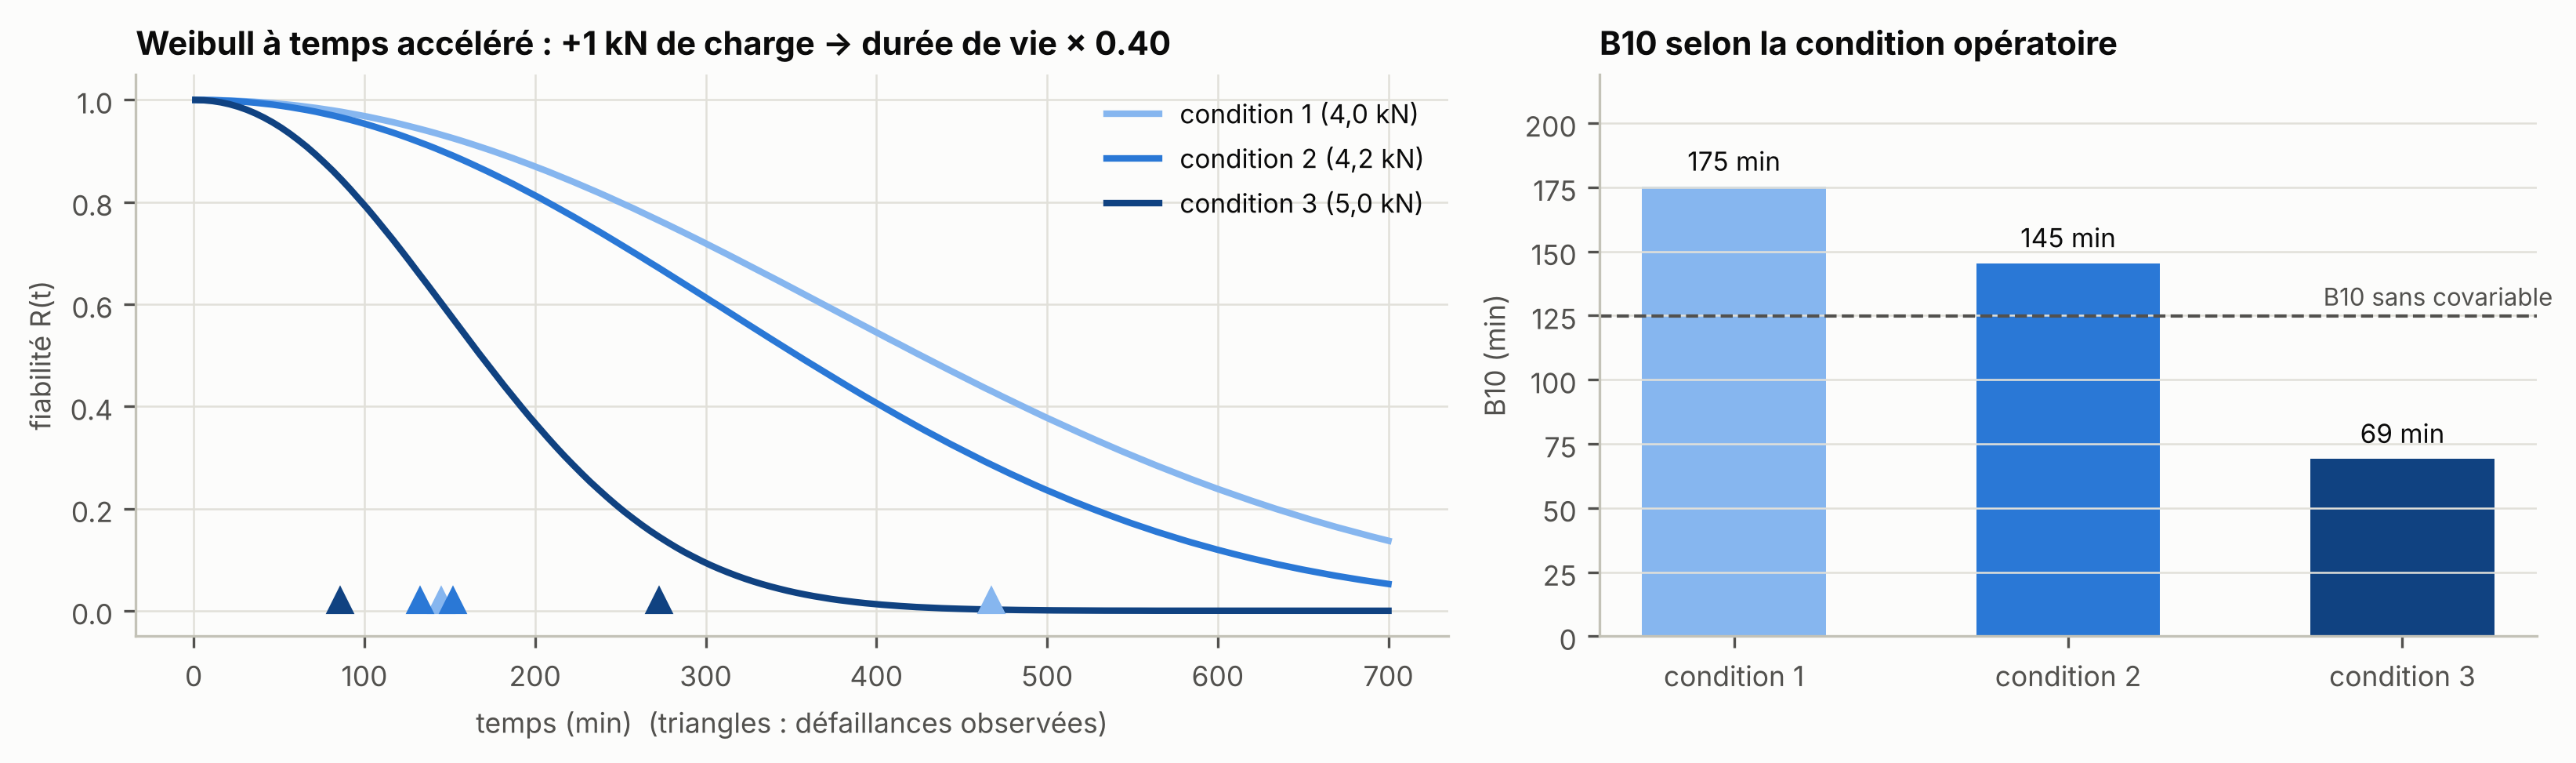
\includegraphics[width=\linewidth]{figures/fig19_covariables.png}
\caption[Effet de la charge (covariable)]{Effet de la charge sur la fiabilité (Weibull à temps accéléré) et B10 par condition.}
\label{fig:covariables}
\end{figure}

\section{Premier défaut et indicateur de santé}

La figure~\ref{fig:fpt} montre la règle des 3 $\sigma$ sur deux roulements : les alarmes passagères sont annulées, et seule l'alarme qui dure est retenue. Sur les 17 roulements, l'alarme arrive en médiane \textbf{7,8 min avant la panne} ; 14 fausses alarmes ont été annulées. À l'instant de troncature du challenge, \textbf{8 roulements de test sur 11 ne montrent encore aucun défaut} : seuls Bearing1\_3, Bearing1\_4 et Bearing3\_3 sont dégradés.

\begin{figure}[H]
\centering
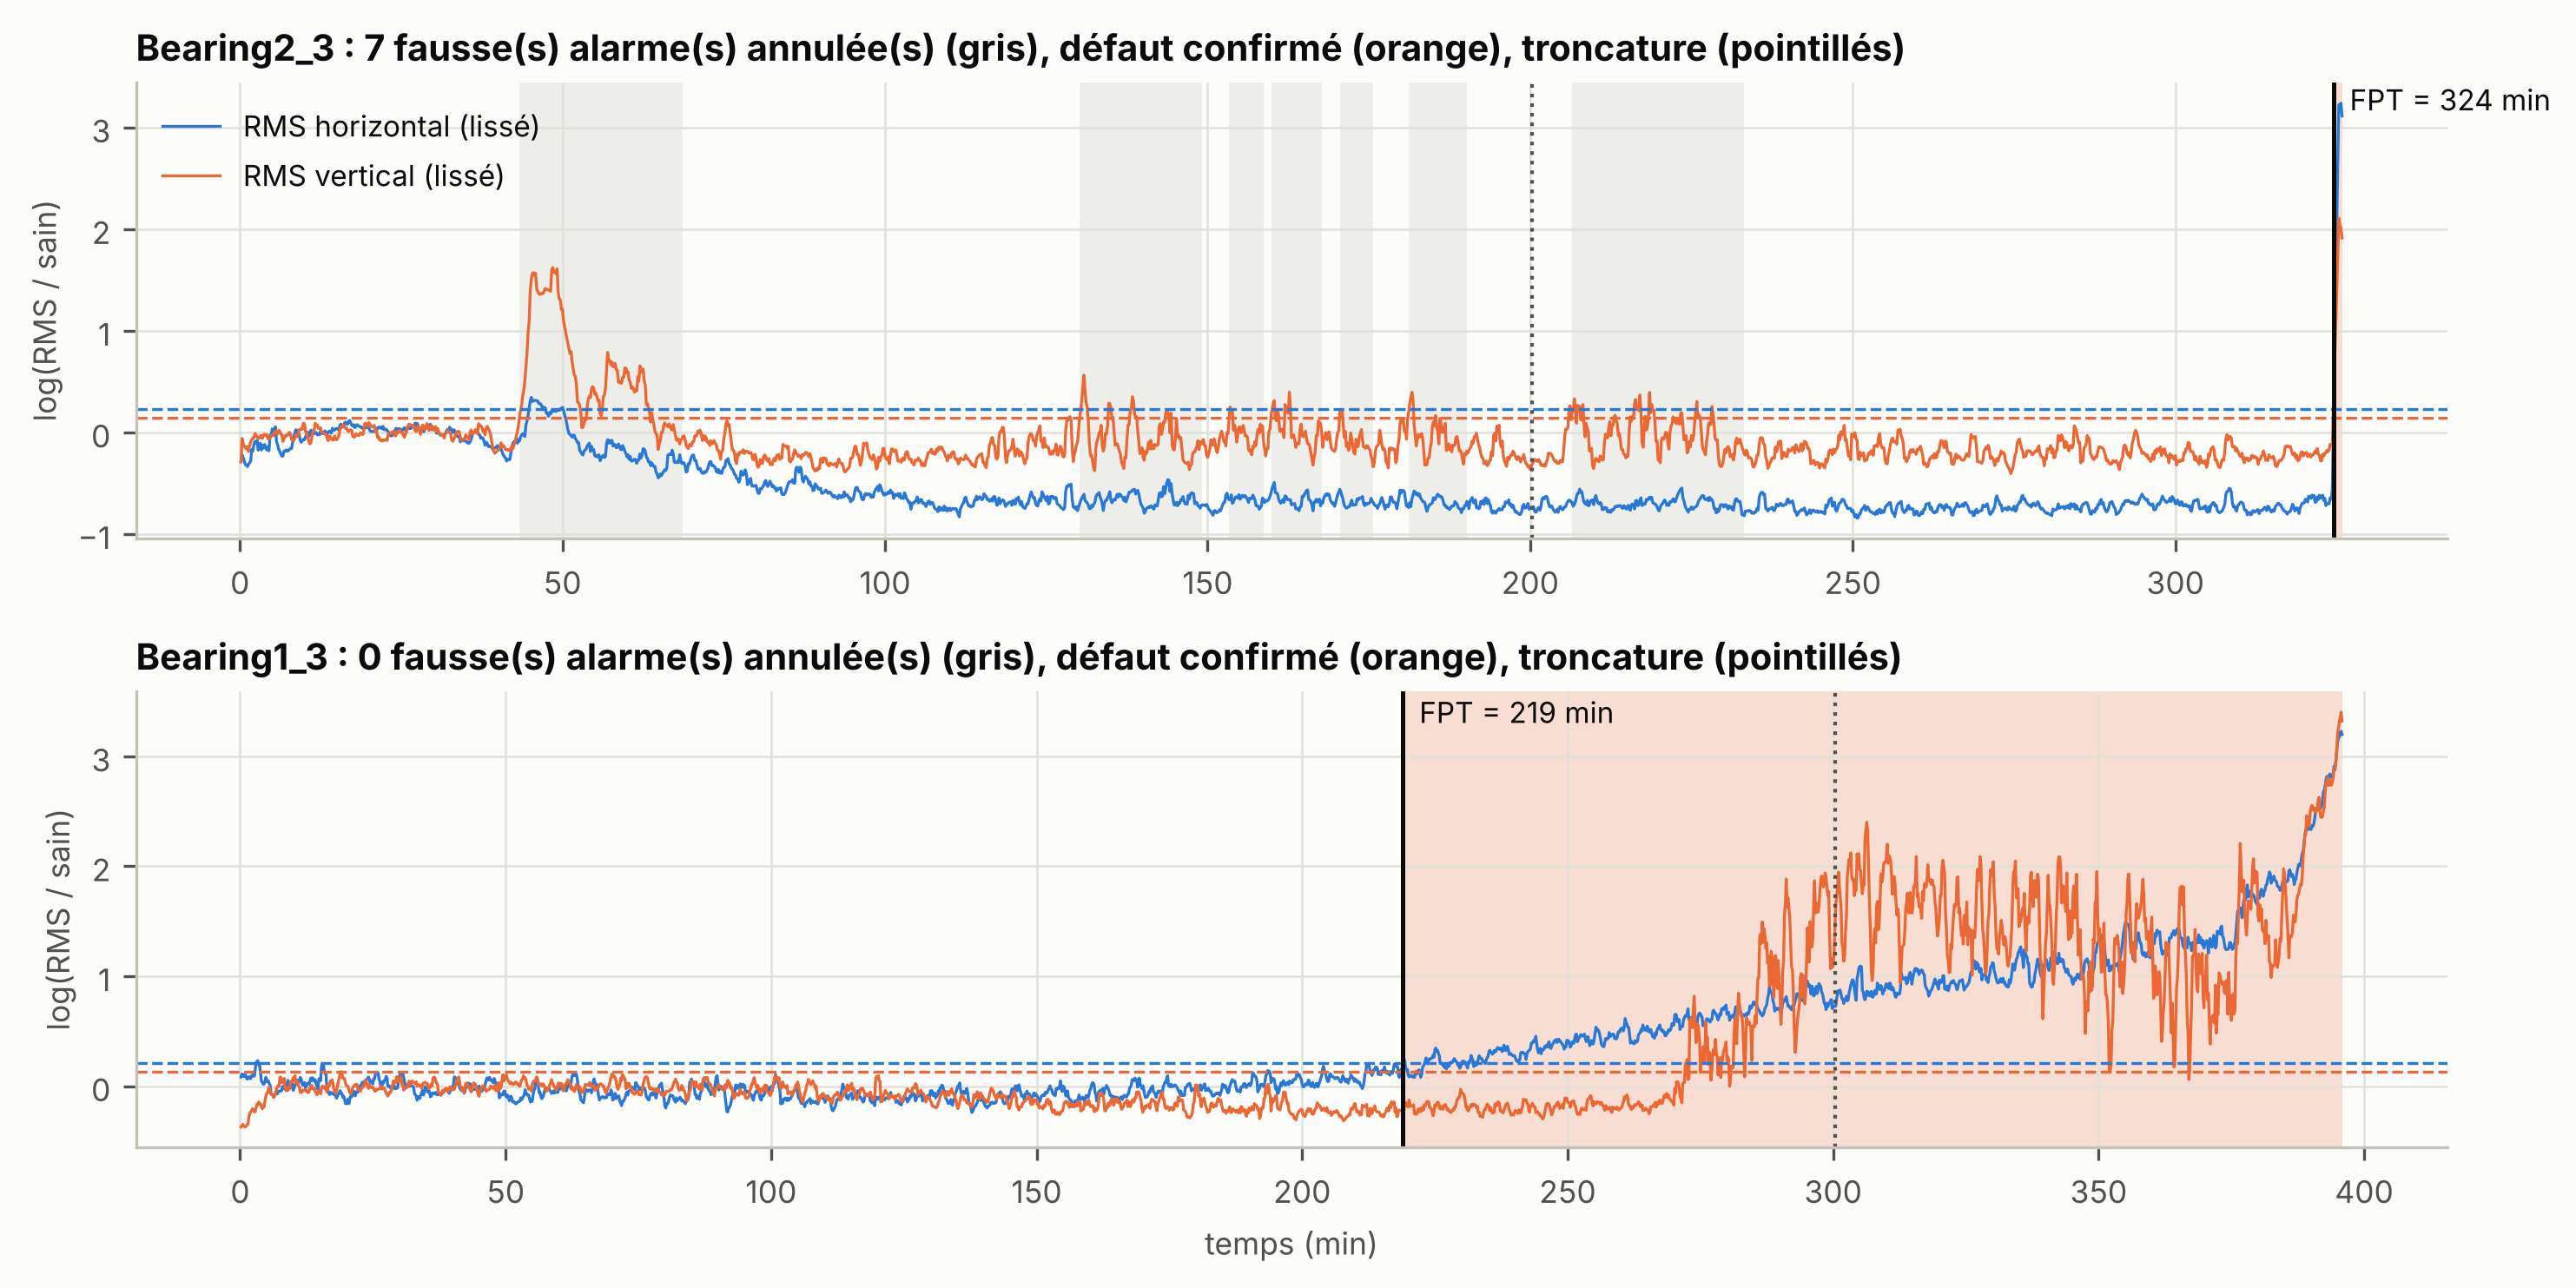
\includegraphics[width=0.86\linewidth]{figures/fig06_detection_fpt.png}
\caption[Détection du premier défaut (règle des 3 $\sigma$)]{Détection du premier défaut par la règle des 3 $\sigma$ (zones grises : fausses alarmes annulées).}
\label{fig:fpt}
\end{figure}

\textbf{Changement du seuil.} Le tableau~\ref{tab:sensibilite} montre l'effet du seuil de détection. Un seuil bas donne plus de fausses alarmes ; un seuil haut prévient plus tard. Le seuil de 3 $\sigma$ est un bon compromis.

\begin{table}[H]
\centering\small
\begin{tabular}{ccccc}
\toprule
Seuil & Fausses alarmes & Délai d'alerte médian & Délai d'alerte moyen & Tests dégradés \\
\midrule
2 $\sigma$ & 25 & 8,0 min & 43,3 min & 3 \\
\textbf{3 $\sigma$} & 14 & 7,8 min & 39,5 min & 3 \\
4 $\sigma$ & 18 & 6,8 min & 30,6 min & 3 \\
5 $\sigma$ & 11 & 6,8 min & 27,0 min & 3 \\
\bottomrule
\end{tabular}
\caption[Sensibilité au seuil de détection]{Sensibilité de la détection au seuil (17 roulements ; dernière colonne : roulements de test déjà dégradés à la troncature).}
\label{tab:sensibilite}
\end{table}

\textbf{Indicateur de santé.} Les 8 meilleures features sont toutes des énergies de bandes d'ondelettes. Le meilleur HI est une seule feature, l'énergie de la bande 6,4–8,0 kHz de l'axe vertical : score 0,644, contre 0,599 pour la moyenne des 8 meilleures. Moyenner rend la fin de vie plus régulière, mais casse la tendance. Le seuil de défaillance vaut $D = 3{,}34 \pm 0{,}63$.

\section{Pronostic de la RUL : benchmark des méthodes}

\subsection{Résultats sur la phase de dégradation}
Le tableau~\ref{tab:resultats} résume les résultats sur les 11 roulements de test. Après le premier défaut, \textbf{toutes les méthodes fondées sur les capteurs battent la fiabilité seule} : RMSE de 16 à 23 min contre 44 min. Le \textbf{processus de Wiener} est le plus précis (RMSE 16,4 min) et le meilleur selon le protocole officiel (score 0,194). Le \textbf{LSTM} a le meilleur score PHM (0,084) : il prédit moins souvent trop tard.

\begin{table}[H]
\centering\small
\begin{tabular}{lccccr}
\toprule
Méthode & RMSE (min) & MAE (min) & Score PHM & Score challenge & Apprentissage \\
\midrule
Fiabilité (B10) & 44,4 & 42,8 & 0,044 & 0,170 & — \\
\textbf{Wiener} & \textbf{16,4} & \textbf{13,0} & 0,059 & \textbf{0,194} & < 0,1 s \\
SVR & 20,0 & 17,1 & 0,059 & 0,175 & 6,5 s \\
GPR & 18,3 & 15,3 & 0,064 & 0,171 & 6,6 s \\
Forêt aléatoire & 23,0 & 18,1 & 0,059 & 0,169 & 14,3 s \\
\textbf{LSTM} & 18,7 & 15,2 & \textbf{0,084} & 0,187 & 200 s \\
CNN 1D & 17,9 & 15,3 & 0,063 & 0,169 & 142 s \\
\bottomrule
\end{tabular}
\caption[Résultats des sept méthodes]{Résultats des sept méthodes sur les 11 roulements de test.}
\label{tab:resultats}
\end{table}

La figure~\ref{fig:trajectoires} montre les RUL prédites au fil du temps sur quatre roulements de test, et la figure~\ref{fig:comparaison} les métriques avec leurs intervalles de confiance.

\begin{figure}[H]
\centering
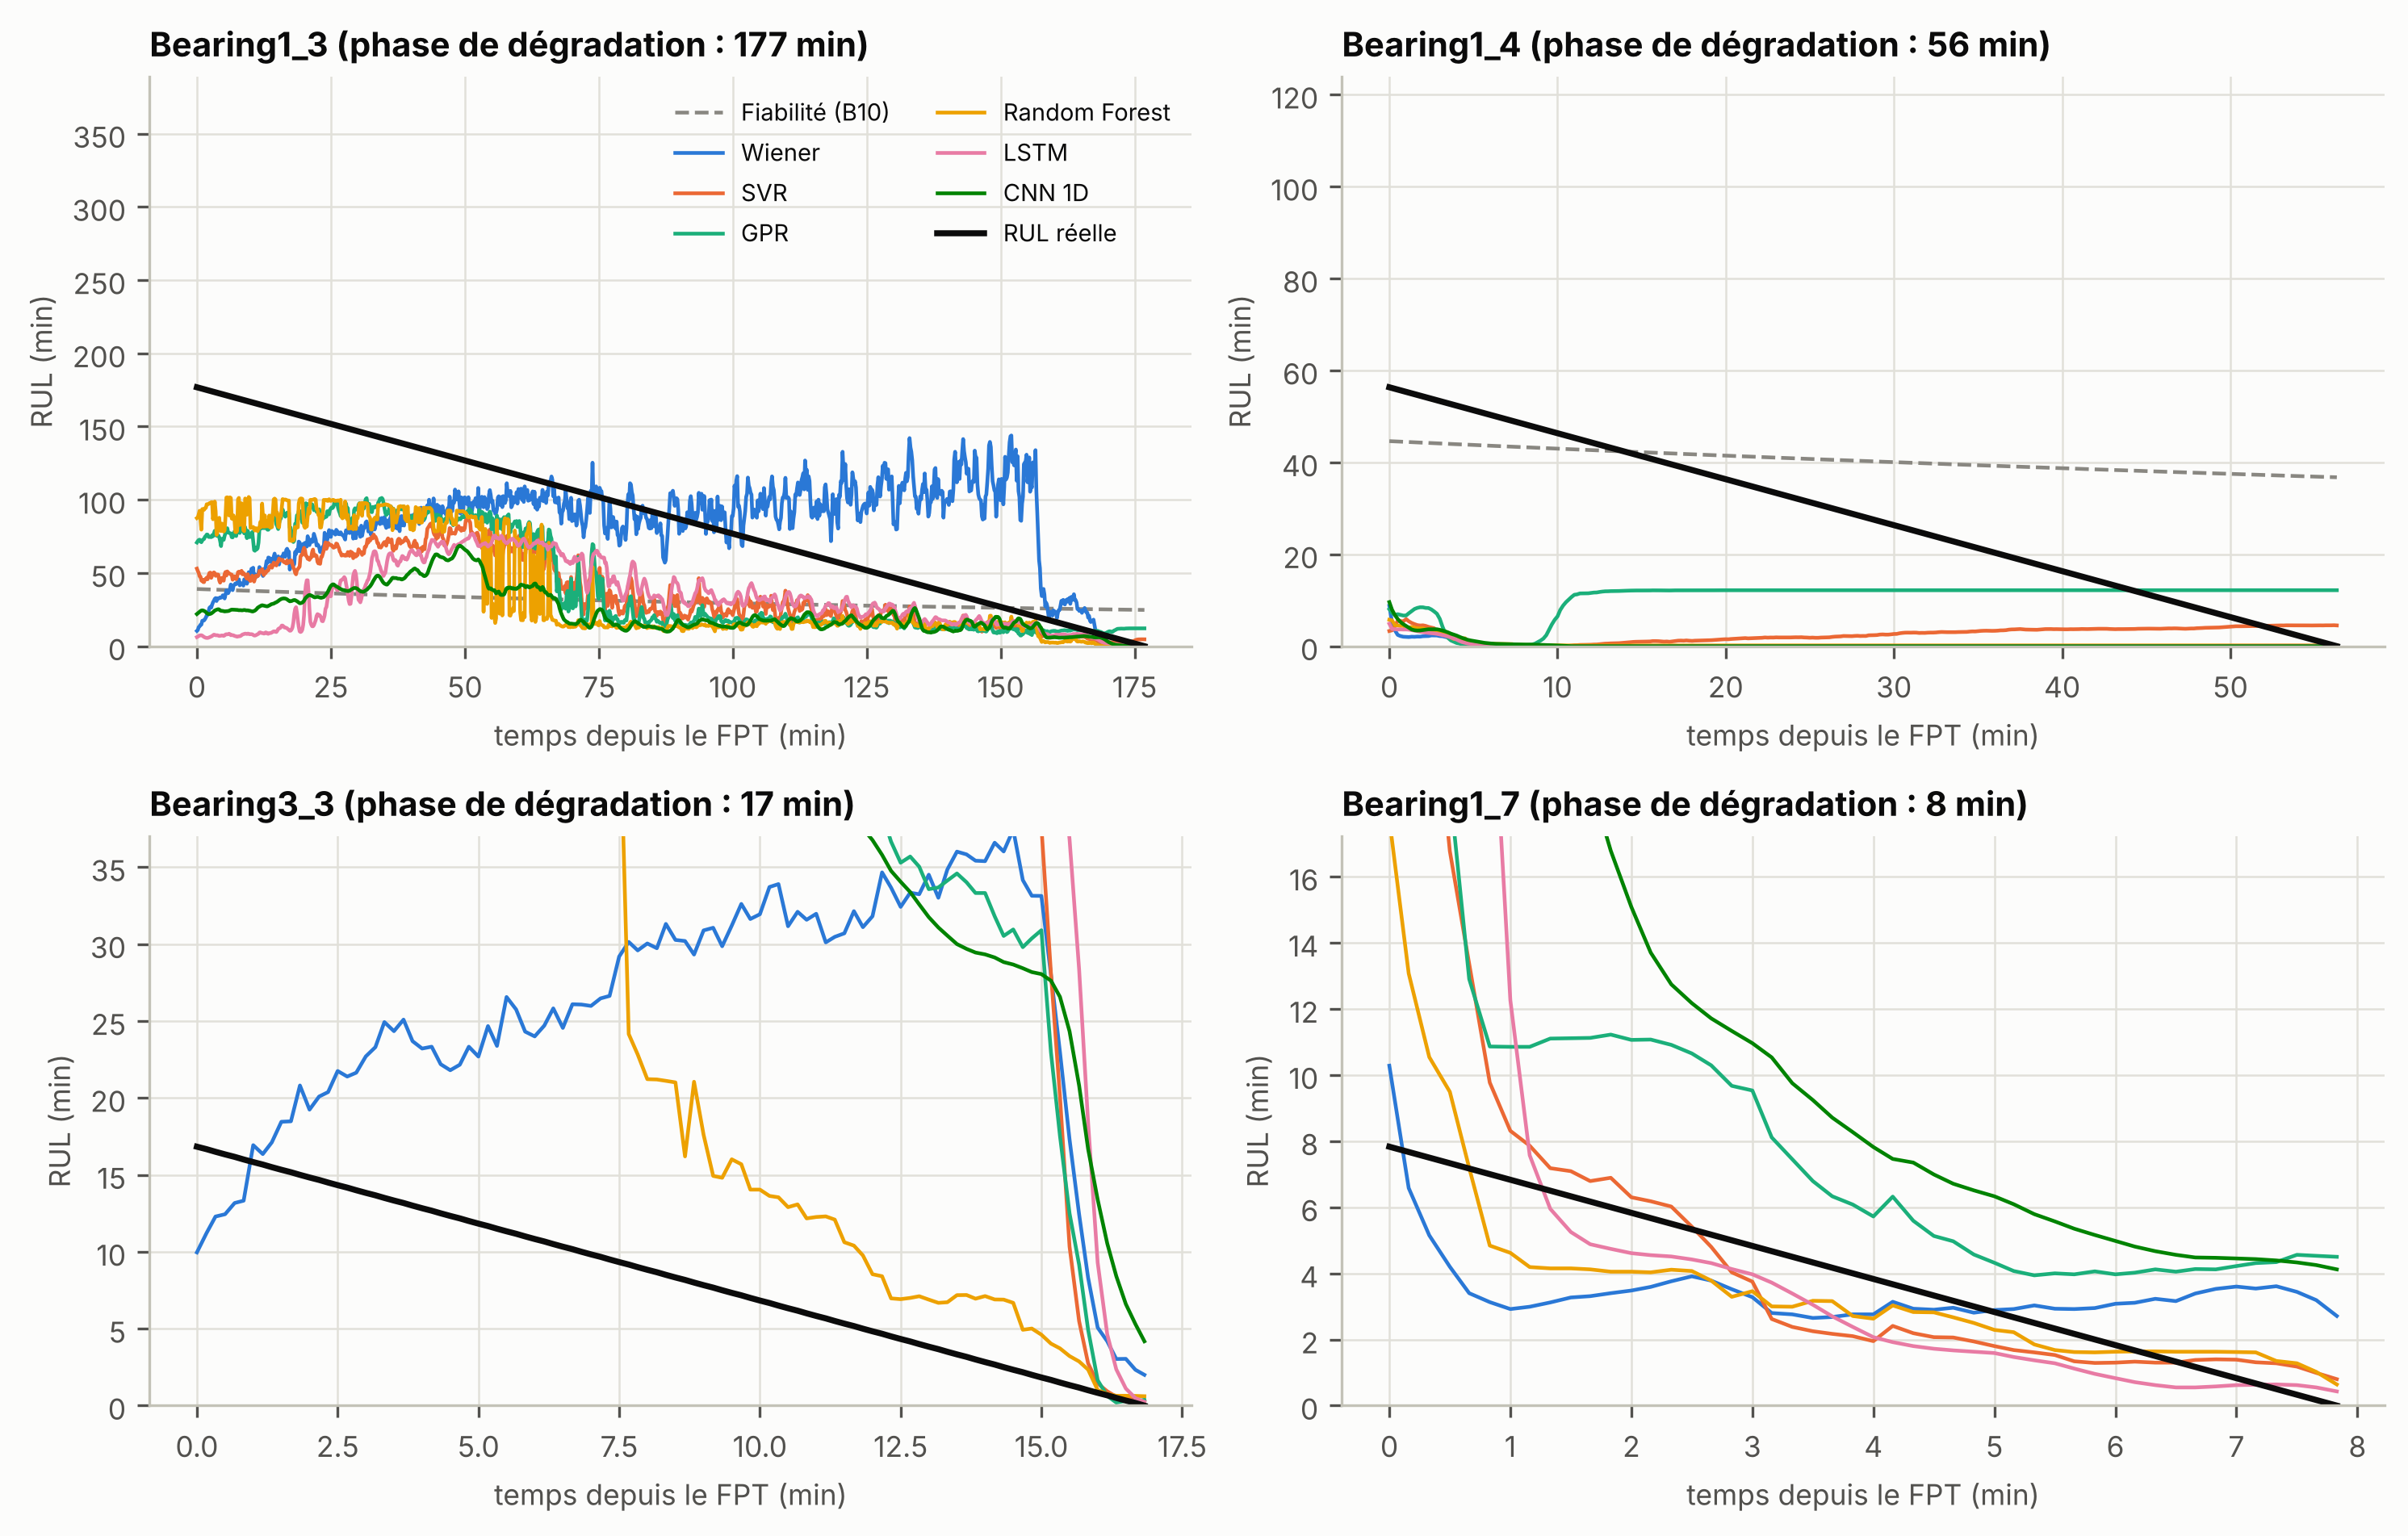
\includegraphics[width=0.86\linewidth]{figures/fig11_trajectoires_rul.png}
\caption[RUL prédite contre RUL réelle]{RUL prédite contre RUL réelle après le premier défaut, sur quatre roulements de test.}
\label{fig:trajectoires}
\end{figure}

\begin{figure}[H]
\centering
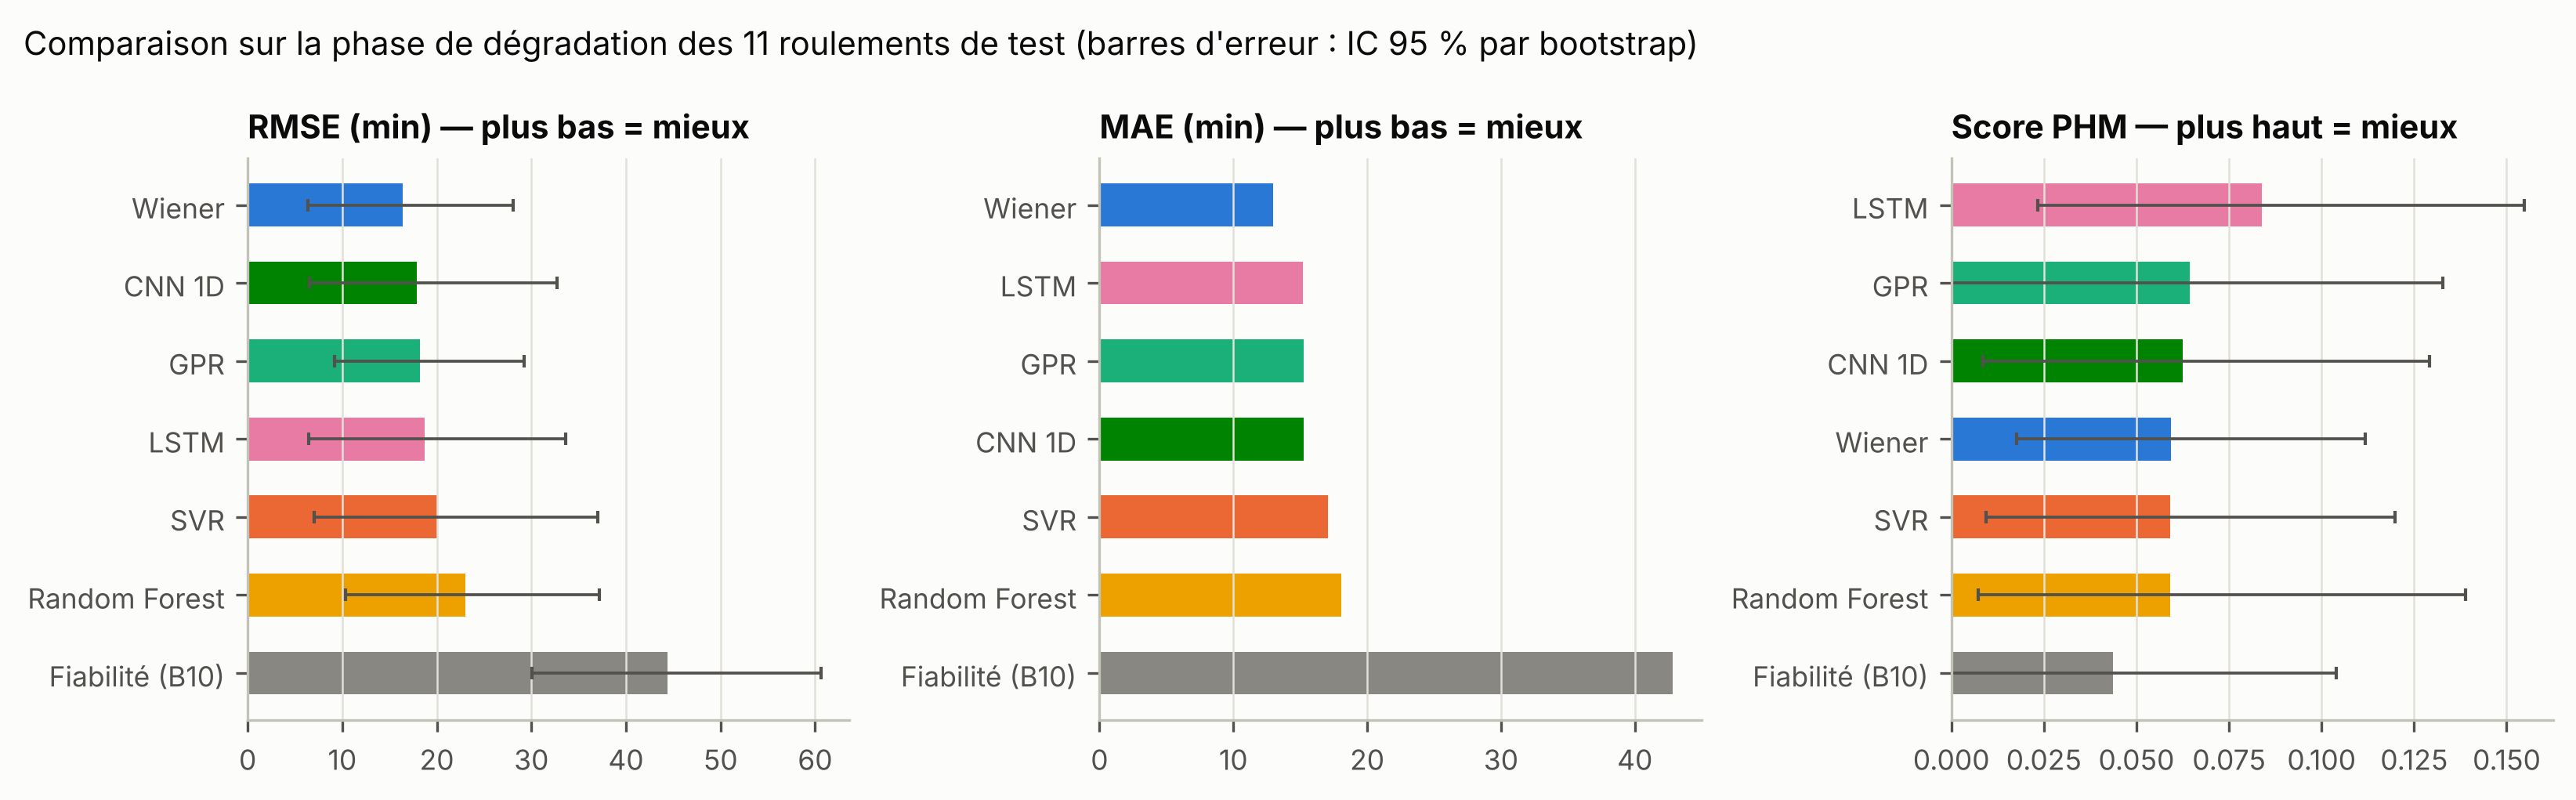
\includegraphics[width=\linewidth]{figures/fig13_comparaison_modeles.png}
\caption[Comparaison des méthodes avec intervalles]{RMSE, MAE et score PHM des sept méthodes (barres d'erreur : IC 95 \% par bootstrap).}
\label{fig:comparaison}
\end{figure}

\subsection{Les écarts sont-ils significatifs ?}
Les intervalles de confiance se chevauchent largement. Le test de Friedman sur les RMSE des 11 roulements donne $p = 0{,}022$ : au moins une méthode se distingue. Le test de Wilcoxon apparié montre que c'est la fiabilité seule : le Wiener la bat sur 9 roulements sur 11 ($p = 0{,}014$). Entre le Wiener et les autres méthodes fondées sur les capteurs, les écarts ne sont pas significatifs ($p$ de 0,21 à 0,70) : \textbf{11 roulements de test ne suffisent pas à les départager}.

\subsection{Benchmark multicritère}
Une méthode ne se juge pas seulement sur sa précision. Le tableau~\ref{tab:benchmark} ajoute la sécurité (prédire trop tard), l'incertitude, l'explicabilité et le coût de calcul.

\begin{table}[H]
\centering\small
\begin{tabular}{lccccc}
\toprule
Méthode & Précision & Sécurité & Intervalle d'incertitude & Explicabilité & Calcul \\
\midrule
Fiabilité (B10) & -- & -- & population & ++ & ++ \\
Wiener & ++ & + & oui & ++ & ++ \\
SVR & + & + & non & -- & + \\
GPR & + & + & possible & -- & + \\
Forêt aléatoire & 0 & + & non & + & + \\
LSTM & + & ++ & non & -- & -- \\
CNN 1D & + & + & non & -- & -- \\
\bottomrule
\end{tabular}
\caption[Benchmark multicritère]{Benchmark multicritère (++ très bon, + bon, 0 moyen, -- faible).}
\label{tab:benchmark}
\end{table}

\subsection{Covariables dans les modèles d'apprentissage}
Nous avons aussi ajouté la charge et la vitesse comme entrées des modèles d'apprentissage automatique (tableau~\ref{tab:covml}). Le GPR progresse sur tous les critères ; le SVR gagne en score mais perd en RMSE ; la forêt aléatoire change peu. Avec seulement 2 roulements d'apprentissage par condition, l'effet reste fragile.

\begin{table}[H]
\centering\small
\begin{tabular}{lcccccc}
\toprule
& \multicolumn{2}{c}{RMSE (min)} & \multicolumn{2}{c}{Score PHM} & \multicolumn{2}{c}{Score challenge} \\
Méthode & sans & avec & sans & avec & sans & avec \\
\midrule
SVR & 20,0 & 22,2 & 0,059 & 0,108 & 0,175 & 0,237 \\
GPR & 18,3 & 17,3 & 0,064 & 0,074 & 0,171 & 0,242 \\
Forêt aléatoire & 23,1 & 22,5 & 0,059 & 0,056 & 0,169 & 0,169 \\
\bottomrule
\end{tabular}
\caption[Covariables dans les modèles d'apprentissage]{Effet des covariables charge et vitesse sur les modèles d'apprentissage (recalcul dans les mêmes conditions).}
\label{tab:covml}
\end{table}

\section{Validation sur données simulées}

Sur des données réelles, on ne connaît jamais toute la vérité. Nous avons donc testé deux méthodes sur des données simulées où la réponse est connue (figure~\ref{fig:simulees}).

\textbf{Loi de Weibull.} On tire des durées de vie dans une Weibull connue ($\beta = 1{,}85$), avec le même plan d'essai que PRONOSTIA (6 essais complets, 11 censurés aux mêmes âges), puis on réestime $\beta$, 400 fois. Avec 17 roulements, $\beta$ estimé va de 1,36 à 3,34 dans 90 \% des cas, avec une légère surestimation en moyenne (2,15) ; avec 204 roulements, il va de 1,66 à 2,11. La méthode est juste, mais \textbf{17 roulements, c'est peu}.

\textbf{Processus de Wiener.} Quand les trajectoires suivent le modèle, l'intervalle à 90 \% contient bien 92 \% des vraies RUL : la méthode est correcte. Un HI qui stagne puis accélère ne la gêne presque pas (92 \%). En revanche, si le seuil de défaillance varie autant que sur les roulements de test (écart-type 1,57 au lieu de 0,63 à l'apprentissage), la couverture tombe à 63 \%, proche des 54 \% observés sur les vraies données. \textbf{Le problème vient du seuil, appris sur 6 roulements seulement, pas du modèle.} D'ailleurs, sans l'incertitude sur le seuil, la couverture réelle tombe à 31 \%.

\begin{figure}[H]
\centering
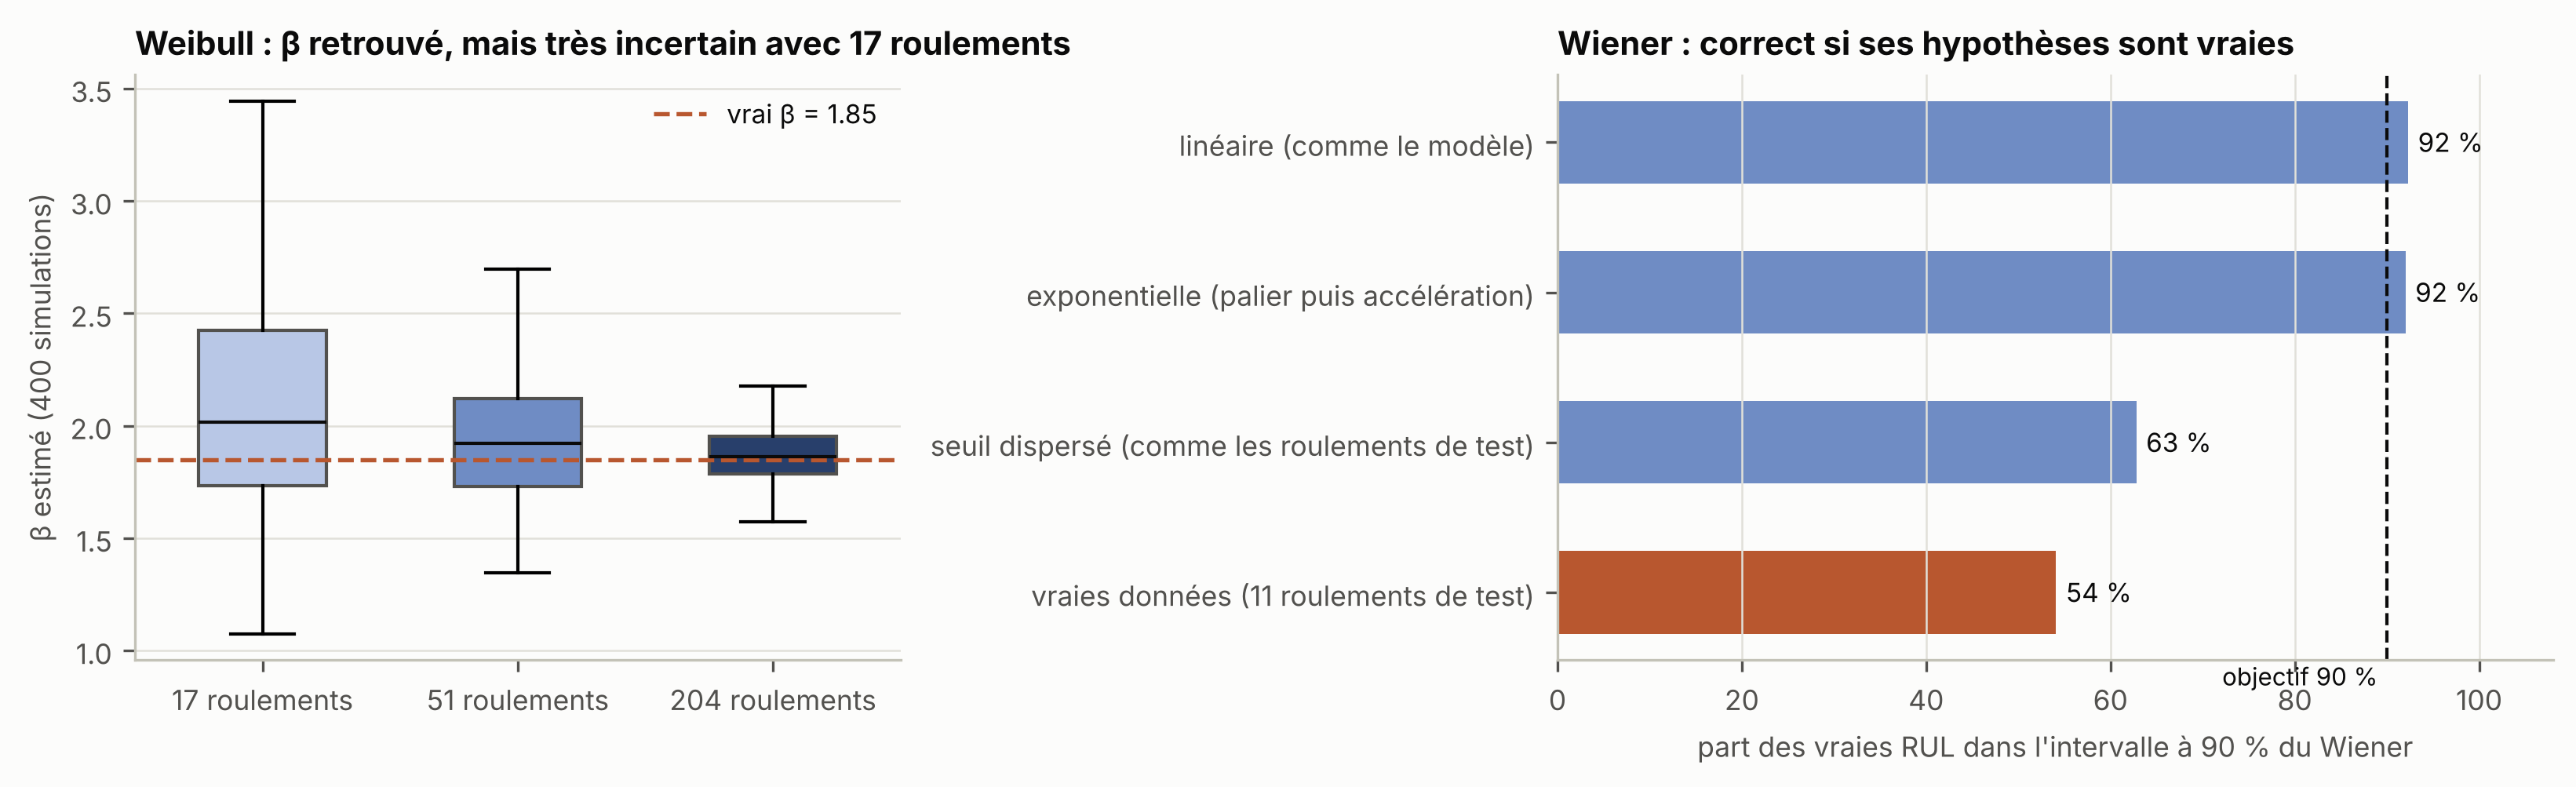
\includegraphics[width=\linewidth]{figures/fig20_donnees_simulees.png}
\caption[Validation sur données simulées]{Validation sur données simulées : estimation de $\beta$ selon le nombre de roulements, et couverture de l'intervalle du Wiener.}
\label{fig:simulees}
\end{figure}

\section{Explicabilité (XAI)}

Pour savoir sur quoi les modèles s'appuient, nous mélangeons au hasard une entrée et regardons de combien l'erreur augmente \cite{breiman2001}. La figure~\ref{fig:xai} montre que les trois modèles utilisent surtout les \textbf{énergies de bandes de fréquence}, et pas seulement le temps écoulé depuis le défaut : ils lisent vraiment l'état du roulement. Les bandes de 1,6 à 9,6 kHz dominent, là où résonnent les chocs d'un défaut. Le processus de Wiener, lui, est explicable par construction : une pente, un seuil, un bruit.

\begin{figure}[H]
\centering
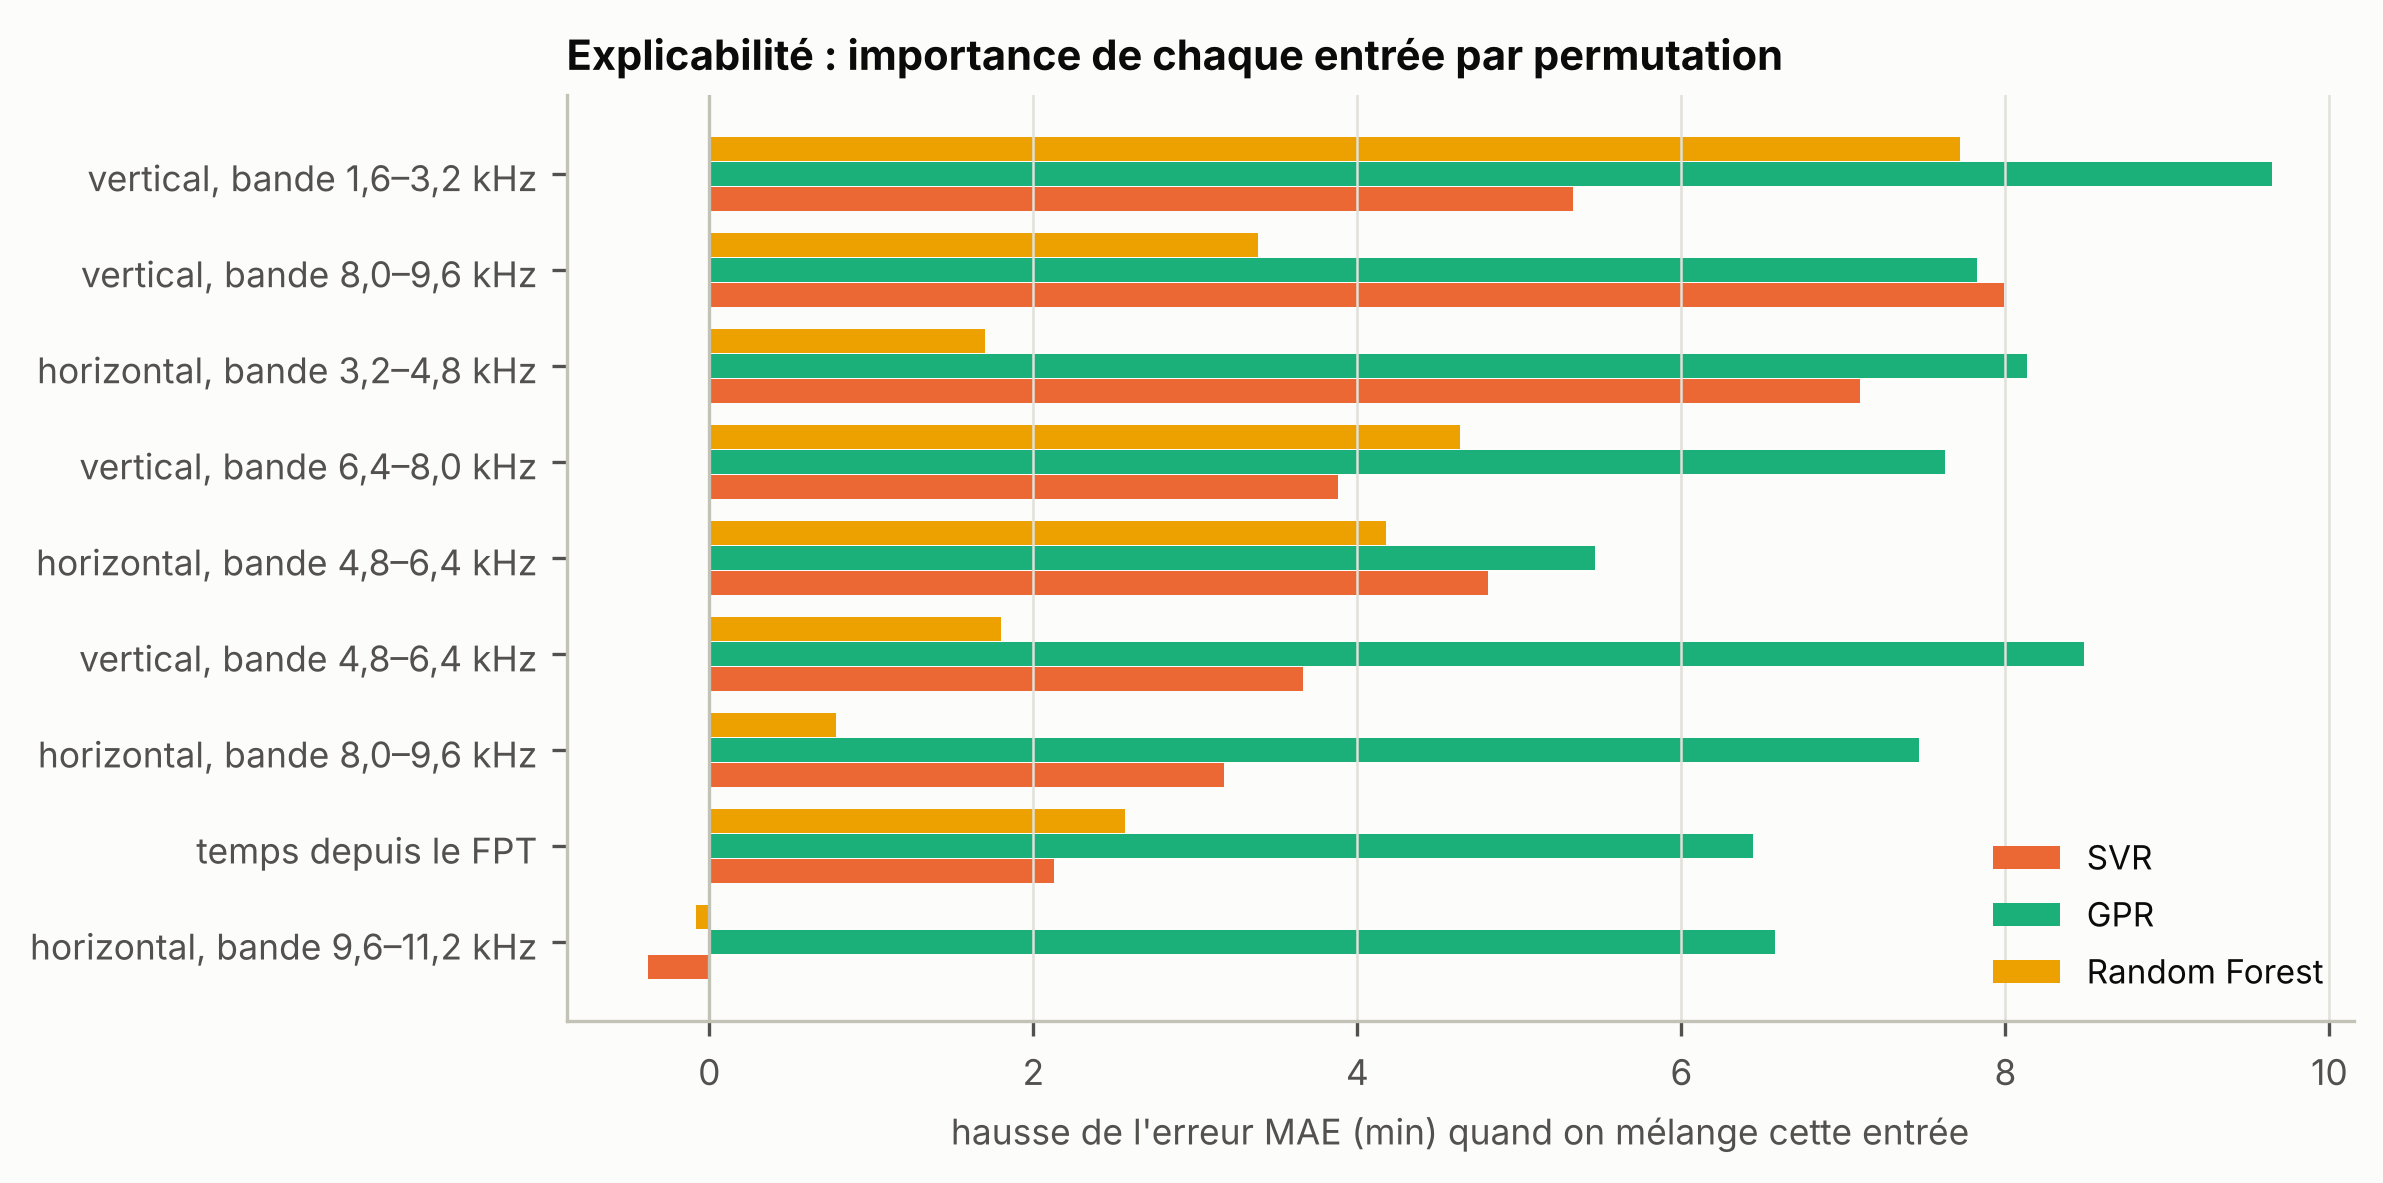
\includegraphics[width=0.72\linewidth]{figures/fig21_xai.png}
\caption[Explicabilité : importance des entrées]{Importance de chaque entrée par permutation, pour le SVR, le GPR et la forêt aléatoire.}
\label{fig:xai}
\end{figure}

\section{Restitution dans un tableau de bord}

Tous les résultats sont présentés dans un tableau de bord interactif en sept pages (figure~\ref{fig:dashboard}) : vue d'ensemble, données et fiabilité, santé et premier défaut, pronostic de la RUL, comparaison des méthodes, décision et économie, tests et validation. Le thème est sombre (noir et bleu), chaque page a sa nuance de bleu, et la page économique permet de changer les coûts en direct.

\begin{figure}[H]
\centering
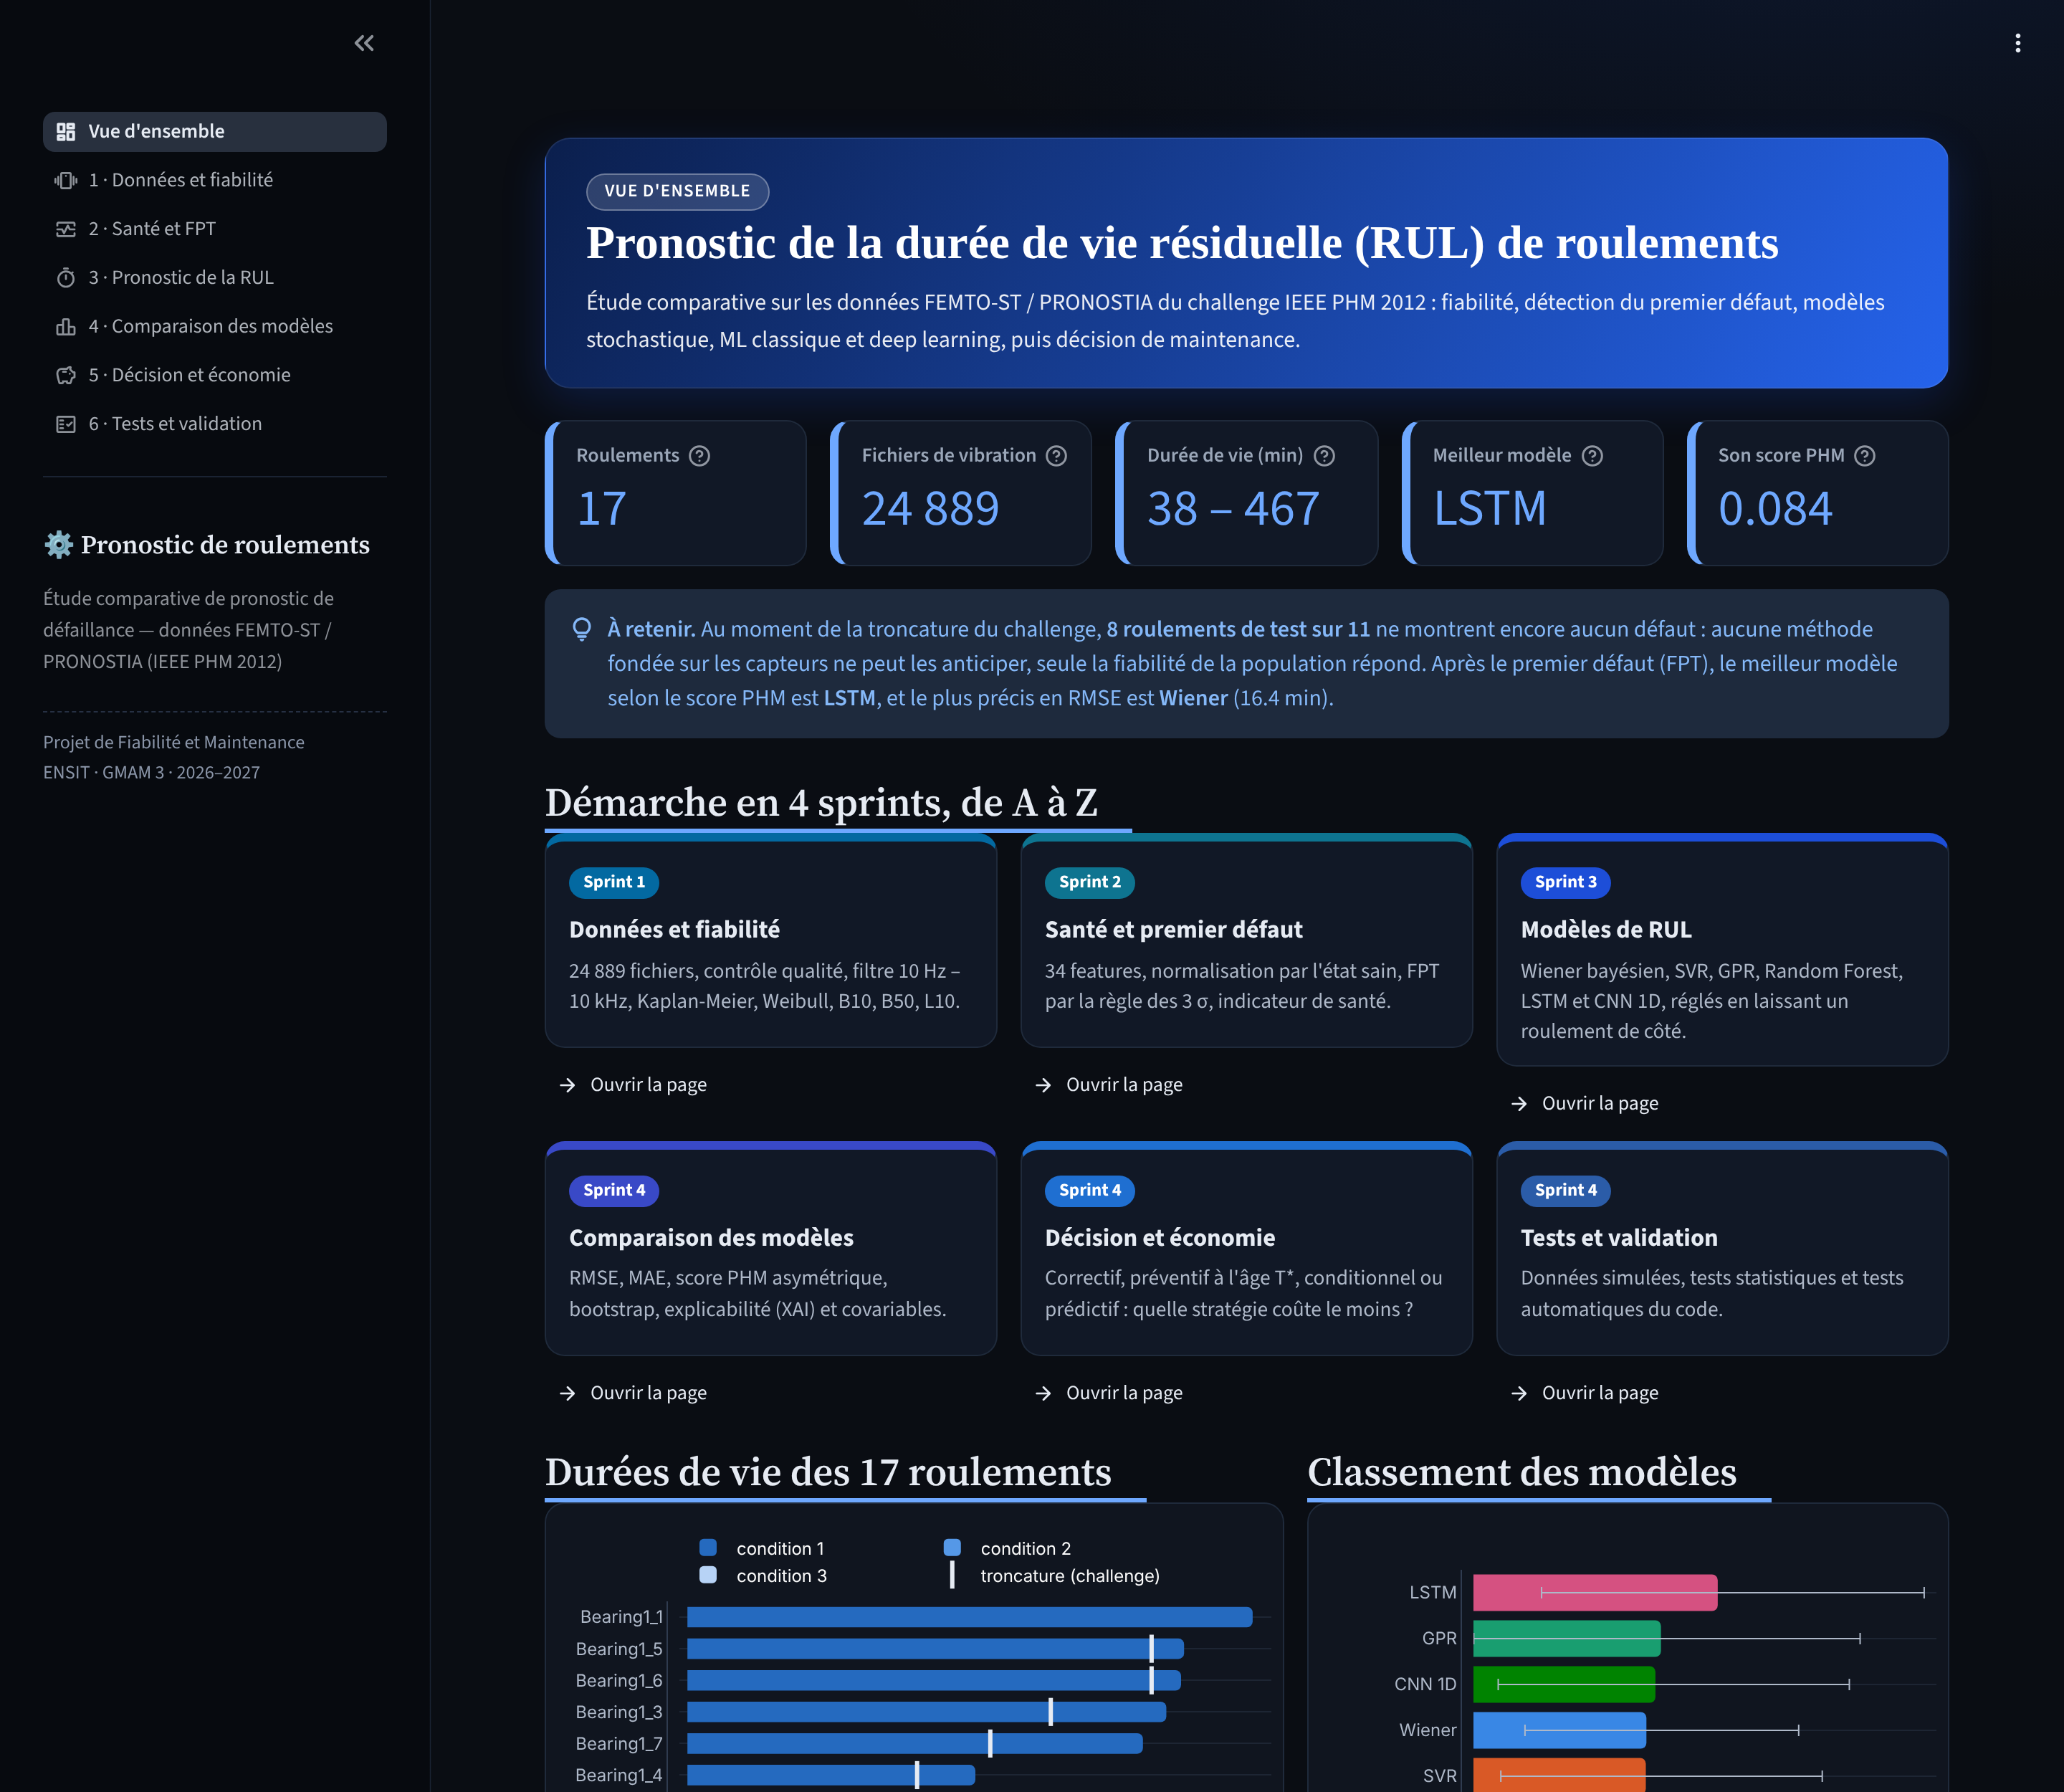
\includegraphics[width=0.7\linewidth]{figures/dashboard_accueil.png}
\caption[Page d'accueil du tableau de bord]{Page d'accueil du tableau de bord (Streamlit) : chiffres clés, démarche et classement des méthodes.}
\label{fig:dashboard}
\end{figure}

\chapconclusion
Après le premier défaut, les capteurs améliorent nettement la prédiction : le Wiener est le plus précis et le LSTM le plus prudent, mais les écarts entre méthodes ne sont pas significatifs avec 11 roulements. Les données simulées montrent que les méthodes sont correctes et que la principale faiblesse vient du seuil de défaillance, appris sur trop peu de roulements.
